%%%%%%%%%%%%%%%%%%%%%%%%%%%%%%%%%%%%%%%%%
% Short Sectioned Assignment
% LaTeX Template
% Version 1.0 (5/5/12)
%
% This template has been downloaded from:
% http://www.LaTeXTemplates.com
%
% Original author:
% Frits Wenneker (http://www.howtotex.com)
%
% License:
% CC BY-NC-SA 3.0 (http://creativecommons.org/licenses/by-nc-sa/3.0/)
%
%%%%%%%%%%%%%%%%%%%%%%%%%%%%%%%%%%%%%%%%%

%----------------------------------------------------------------------------------------
%	PACKAGES AND OTHER DOCUMENT CONFIGURATIONS
%----------------------------------------------------------------------------------------

\documentclass[paper=a4, fontsize=11pt]{article} % A4 paper and 11pt font size
\usepackage[margin=0.7in]{geometry}
\usepackage[T1]{fontenc} % Use 8-bit encoding that has 256 glyphs
%\usepackage{fourier} % Use the Adobe Utopia font for the document - comment this line to return to the LaTeX default
\usepackage[francais]{babel} % English language/hyphenation
\usepackage[utf8]{inputenc}
\usepackage[babel=true]{csquotes} 
%\usepackage{amsmath,amsfonts,amsthm}
%\usepackage{algorithmicx} % Math packages
\usepackage{algorithm}
\usepackage[noend]{algpseudocode}
\usepackage{lipsum} % Used for inserting dummy 'Lorem ipsum' text into the template
\usepackage{float}
\usepackage{graphicx}
%----------------------------------------------------------------------------------------
%	TITLE SECTION
%----------------------------------------------------------------------------------------

\newcommand{\horrule}[1]{\rule{\linewidth}{#1}} % Create horizontal rule command with 1 argument of height

\title{	
\normalfont \normalsize 
\textsc{Master SAR} \\ [25pt] % Your university, school and/or department name(s)
\horrule{0.5pt} \\[0.4cm] % Thin top horizontal rule
\huge Projet ARA \\ % The assignment title
\horrule{2pt} \\[0.5cm] % Thick bottom horizontal rule
}

\author{Alexandra Hospital, Thomas Medioni} % Your name

\date{\normalsize\today} % Today's date or a custom date

\begin{document}

\maketitle % Print the title

\pagenumbering{arabic}
\newpage

%----------------------------------------------------------------------------------------
%	EXERCICE 1
%----------------------------------------------------------------------------------------

\section{Exercice 1}

\subsection{Question 1}

L'article traite des problèmes d'élection de leader au sein d'un système mobile ad hoc. En utilisant l'algorithme d'arbres couvrants de Dijkstra et Scholten dans les réseaux statiques et en l'adaptant aux problématiques des réseaux mobiles ad hoc, dans lequel l'état des composantes connexes n'est pas assuré dans le temps, les auteurs fournissent un algorithme permettant d'assurer à terme un leader unique par composante connexe.
Le taux d'élection est supérieur à 95\% en fonction de l'algorithme de transport.

\subsection{Question 2}

L'algorithme fait les hypothèses suivantes sur le système :
\begin{itemize}
\item Il est modélisable par un graphe dynamique non orienté dont les noeuds sont mobiles et les arêtes représentent l'existence d'une connexion entre deux noeuds, c'est-à-dire la capacité pour un noeud à communiquer directement avec un autre.

\item Chaque noeud possède une valeur exprimant son aptitude à être leader ainsi qu'un identifiant unique et ordonné. La valeur du noeud la plus élevée représente le noeud le plus apte à être leader, l'identifiant unique sert à départager deux candidats à aptitudes égales.

\item Les canaux de communication entre les noeuds sont bidirectionnels et respectent un ordre FIFO entre deux noeuds adjacents.

\item La mobilité des noeuds peut impliquer des changements de topologie entraînant des partitions ou des fusions du réseau. De plus, les noeuds peuvent crasher de manière arbitraire .

\item Les messages ne sont délivrés que si l'émetteur et le récepteur sont connectés durant l'émission du message.

\item Les buffers de réception sont infiniment larges de manière à ce que il n'y ait jamais de dépassement de capacité.

\item Les communications s'effectuent par échange de messages point-à-point de manière asynchrone.

\end{itemize}

\newpage
\subsection{Question 3}

Les élections concurrentes au sein d'une même composante connexe sont gérées grâce au couple de valeurs \\ \textit{<num, id>} selon la règle suivante :\\
Soient \textit{<num1, id1>} et\textit{<num2, id2>} deux indexes de noeuds concurrents. Le noeud possédant le num le plus grand l'emporte.
Si num1 = num2, le noeud qui a le plus grand identifiant l'emporte.

C'est le consensus : tous les noeuds s'accordent sur un noeud qui lancera l'élection (qui sera la racine de l'arbre).


\subsection{Question 4}

\textbf{Processus i :}
\newline
Variables locales : 
\newline
$ N_{i} $ : tableau de voisins 
\newline
$ S_{i} $ : tableau de voisins dont on attend encore un message ack (initialisé à \textit{null})
\newline
$ parent_{i} $ : père du noeud
\newline
\begin{algorithm}[H]
   \caption{Leader\_election()}
    \begin{algorithmic}[1]

%%%%%%%%%%%%%%%%%%%%%%%%%%%%%%%%%%%%%%%%%%%%%%%%%%%%%%
% ---------------- leader_election() ----------------%
%%%%%%%%%%%%%%%%%%%%%%%%%%%%%%%%%%%%%%%%%%%%%%%%%%%%%%

      \Function{leader\_election}{}\Comment{}
		\If {$i == source$}
			\State $ send <election, i>$ to $ N_{i}$
		\EndIf
       \EndFunction

%%%%%%%%%%%%%%%%%%%%%%%%%%%%%%%%%%%%%%%%%%%%%%%%%%%%%%
% --------- upon_reception(<election, j) ------------%
%%%%%%%%%%%%%%%%%%%%%%%%%%%%%%%%%%%%%%%%%%%%%%%%%%%%%%

      \Function{upon reception}{<election, j>}\Comment{}
		\If {$parent == null $}
			\State $parent \gets j$
			\State $ S_{i} \gets N_{i} \setminus parent $
			\State $ send <election, i>$ to $ S_{i}$

			\While {$ S_{i}$ is not empty } 
				\State  wait until receive <ack ,s>
				\State   upon reception <ack, s> 
				\State $ S_{i} \gets S_{i}\setminus s $ 
			\EndWhile

		\EndIf
		\State  send <ack, i> to \textit{parent}
       \EndFunction

%%%%%%%%%%%%%%%%%%%%%%%%%%%%%%%%%%%%%%%%%%%%%%%%%%%%%%
% ------------- upon_reception <ack, j> --------------%
%%%%%%%%%%%%%%%%%%%%%%%%%%%%%%%%%%%%%%%%%%%%%%%%%%%%%%

      \Function{upon reception}{<ack, j>}\Comment{}
			\State $ S_{i} \gets S_{i}\setminus j $ 
       \EndFunction


%%%%%%%%%%%%%%%%%%%%%%%%%%%%%%%%%%%%%%%%%%%%%%%%%%%%%%
% ----------- upon_reception <leader, j> ------------%
%%%%%%%%%%%%%%%%%%%%%%%%%%%%%%%%%%%%%%%%%%%%%%%%%%%%%%

      \Function{upon reception}{<leader, j>}\Comment{}
			\State $ send <leader, i> $ to $  N_{i} \setminus \textit{parent} $
       \EndFunction
\end{algorithmic}
\end{algorithm}
%
%upon reception <election, j>
%	if parent == null
%		parent = j
%		Si = Ni \ parent
%		send <election, i> to Si
%		while (Si not empty)
%			wait unti receive <ack, s>
%			upon reception <ack, s>
%			Si = Si \ s
%
%	send <ack, i> to parent
%			
%
%upon reception <ack, j>
%	Si = Si \ j
%
%upon reception <leader, j>
%	send <leader, i> to Ni \ parent
%
%
Complexité en messages : O(n)
Chaque noeud envoie un message Election à tous ses voisins sauf son parent et attend un ack d'eux.
Le noeud source "broadcast" la valeur du leader.

 
\subsection{Question 5}
C'est le système de heartbeat avec temporisation : si on ne reçoit pas de message \enquote{je suis en vie} d'un noeud depuis un certain temps borné, on considère qu'il est en panne. 

\subsection{Question 6}

Le modèle de mobilité Random Waypoint est utilisé pour simuler les changements de position, vitesse, et accéleration en fonction du temps. Ce modèle est fortement utilisé
pour étudier les comportements des noeuds au sein des MANET. Chaque noeud est d'abord immobile pendant un nombre fixé de secondes, puis choisit une destination aléatoire, ainsi qu'une vitesse aléatoire choisie entre une borne
minimum et maximum. Le noeud se déplace alors jusqu'à sa destination puis effectue une pause avant de choisir une nouvelle destination et une nouvelle vitesse de manière aléatoire. Ce comportement est observé par tous les noeuds jusqu'à 
la fin de la simulation.

\newpage
\section{Exercice 2}
Dans cette section, nous allons expliquer nos choix d'implémentation des algorithmes de l'exercice 2.

\subsection{Question 1}
Classe RandomWayPointProtocol.java \\
Chaque noeud va tirer aléatoirement sa position x et y de départ et de destination, puis calculer sa prochaine position à partir de sa vitesse. 

\subsection{Question 2}
Classe EmitterImpl.java\\
La méthode d'émission envoie un message à chaque noeud qui fait partie de ses voisins, c'est-à-dire qui est à une distance inférieure à la portée.

\subsection{Question 3}
Classe ElectionProtocolImpl.java \\
Pour implémenter les messages Probe, nous avons décidé d'utiliser une liste supplémentaire pour stocker les noeuds en vie : ceux dont on a reçu un message Probe depuis le dernier delta. On vide cette liste tous les delta temps.
A chaque timer delta, on va faire la différence entre la liste de voisins et la liste des noeuds en vie. Si un noeud n'est pas dans la liste des noeuds en vie, cela signifie qu'on n'a pas reçu de message Probe depuis delta temps au moins, donc il n'est plus considéré comme un voisin.
On ajoute ensuite dans la file d'événements un événement différent des messages pour se \enquote{réveiller} au bout de delta temps.


\subsection{Question 4}
Chaque noeud tire sa valeur de décision aléatoirement. Pour cela nous avons défini une valeur maximum dans le fichier de configuration.\\
Un noeud qui n'a pas de leader lance une élection.

Lorsqu'on reçoit un message élection d'un noeud qui n'est pas notre parent, cela signifie qu'une élection à laquelle on fait partie a déjà commencé : on renvoie donc un ack à ce noeud.
Nous avons donc besoin de différencier un ack d'un noeud \enquote{cousin} d'un ack d'un noeud \enquote{enfant}, lorsqu'on remonte l'arbre à partir des feuilles.
Ici nous avons choisi de renvoyer la valeur de décision -1 lorsque l'ack vient d'un noeud qui n'est pas notre enfant. 

Si un noeud sort de notre réseau alors qu'on lui a envoyé un message élection, on va attendre son ack indéfiniment. 
Pour résoudre ce problème, lors du traitement de l'événement \enquote{delta}, lorsqu'un noeud sort de nos voisins on le supprime également de la liste des noeuds dont on attend un ack.

Perte du parent : à chaque Ack émis on envoie aussi sa value. Donc chaque noeud qui reçoit un Ack qu'il attend doit comparer la valeur maximale appelée leaderValue à la valeur reçue, ainsi qu'à sa valeur, pour ne garder que la plus grande (c'est celle qui déterminera qui est le leader). On garde également l'id du noeud qui a remporté cette comparaison de valeur.

Un noeud qui a reçu tous les Ack qu'il attendait et qui n'a pas de parent est le noeud qui a initialisé l'élection : c'est lui qui doit diffuser le message leader à tout le monde. Pour cela on considère que si la variable parent est à -1, cela signifie qu'on n'a pas de parent.

Réception du message Leader :
Si on est en élection, on met à jour notre idLeader, on diffuse le message leader à tous les noeuds de notre portée. On n'est plus en éléction, on a fini.


Lancement de l'algo : newElection()
Dans le monitor, on envoie un message élection particulier avec un objet dans le "content". A la reception de ce message dans le processEvent, chaque noeud va commencer une nouvelle élection.

\subsection{Question 5}
Pour gérer la détection de la perte du leader, comme on attend un Probe message de tous nos voisins, on regarde si ce Probe message vient du leader (c'est-à-dire du noeud qui a gagné l'élection, comme expliqué précedemment).
Dans ce cas on fait suivre ce message.
Dans le cas où on ne reçoit pas ce message \enquote{probe leader} du leader, cela signifie qu'on l'a perdu et il faut relancer une élection.
Ce message est différencié des autres car on envoie une valeur Long dans l'object, alors que pour les autres cette valeur sera à null.
Ce message est propagé dans tout le réseau, donc pour éviter qu'il boucle indéfiniment dans le réseau et fausse la détection de la perte du leader, on a ajouté un numéro de séquence lié au message.
A chaque nouveau delta, on incrémente ce numéro de séquence \textit{seqNum} dans la classe ProbeMessage.
Lorsqu'on reçoit ce message, si le numéro de séquence est plus grand que celui qu'on avait (initialement 0), c'est un nouveau heartbeat du leader, on le prend en compte.
Sinon, c'est un message qu'on a déjà reçu, on l'ignore. Réciproquement, le leader qui envoie son heartbeat incrémente ce compteur à chaque delta.

Désormais, chaque noeud qui n'a plus de contact avec son leader va lancer une nouvelle élection.
\newpage
\section{Exercice 3}

\subsection{Question 1}
MetricsController et NbLeaderController


F : A chaque élection, on mesure le temps à partir du début de l'élection jusqu'à ce que le noeud ait un leader puis on calcule le pourcentage. \newline
R : Pour chaque noeud, on calcule le nombre d'élections différentes auxquelles il participe, puis on fait la moyenne sur une unité de temps (une minute dans nos exécutions). \newline
T : Pour chaque noeud, on calcule le temps moyen passé dans une élection, et on divise par le nombre d'élections. \newline
M : On incrémente une variable qui mesure le nombre de messages envoyés (hors Probe Message, car on a considéré qu'ils n'étaient pas vraiment des messages d'élection), puis on divise par le nombre d'élections.
L : A chaque step, on compte le nombre de leaders qu'il y a et on fait la moyenne sur l'exécution.

Pour R, T et M on fait la moyenne sur chaque noeud, puis on divise par le nombre de noeuds du réseau pour avoir la moyenne sur toute l'exécution.

On calcule pour chaque valeur sur un noeud son écart à la moyenne.
%----------------------------------------------------------------------------------------


\subsection{Question 2}

Pour nos tests :\newline
Seed 7\newline
endtime 72000000 \newline
height 2000 \newline
width  2000 \newline
timeout 1000\newline
pause 10000\newline

\newpage
\begin{figure}[!h]
\centering
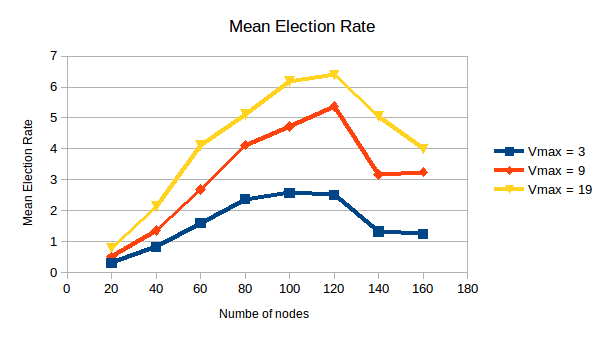
\includegraphics[width=\textwidth]{mean_election_rate.png}
\caption{Mean Election Rate}
\label{MER}
\end{figure}
Comme dans l'article, sur l'ensemble des courbes, le nombre d'élections augmente jusqu'à un certain seuil (120 noeuds sur notre graphique), puis diminue avec l'augmentation du nombre de noeuds. Cela est dû au fait qu'avec un petit nombre de noeuds, beaucoup de noeuds sont isolés. Quand le nombre de noeuds augmente, les noeuds isolés vont rencontrer d'autres noeuds isolés et donc relancer des élections. Cela va former des petites composantes connexes. A partir d'un certain nombre de noeuds, une majorité des noeuds vont être connectés entre eux et donc ils n'auront plus besoin de lancer d'élection.

L'allure des courbes est similaire à celle de l'article, mais les valeurs sont différentes, ce qui peut être dû aux valeurs que nous avons choisi pour le \textit{timeout}.


\newpage
\begin{figure}[!h]
\centering
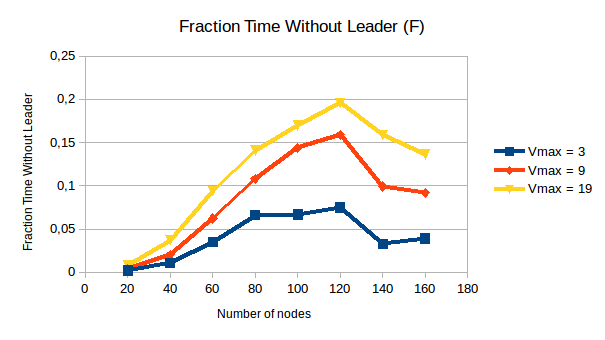
\includegraphics[width=\textwidth]{fraction_time_without_leader.png}
\caption{Fraction Time Without Leader}
\label{FTWT}
\end{figure}

Ici, nous avons obtenu des allures de courbes complètement différentes de celles de l'article. Cela est probablement dû à la valeur de notre \textit{timeout}.

\begin{figure}[!h]
\centering
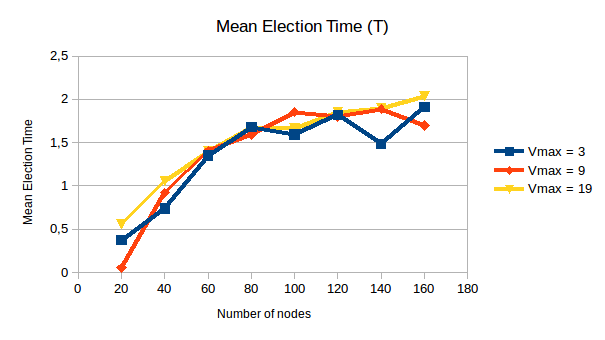
\includegraphics[width=\textwidth]{mean_election_time.png}
\caption{Mean Election Time}
\label{MET}
\end{figure}

Les trois courbes sont croissantes, car plus le nombre de noeuds augmente et plus de noeuds feront partie d'une élection.

\subsection{Question 3}
Les valeurs obtenues en utilisant comme variable du système la vitesse maximale des noeuds et le nombre de noeuds font une hypothèse forte sur l'environnement de simulation : l'espace est limité. Or, les variations de comportement dues au nombre de noeuds sont en fait dues à la densité de la simulation. 
Il est plus pertinent de parler de densité que de nombre de noeud car on inclut la notion de largeur-longueur dans la densité. L'expérience peut donc passer à l'échelle.

\subsection{Question 4}

\begin{figure}[!h]
\centering
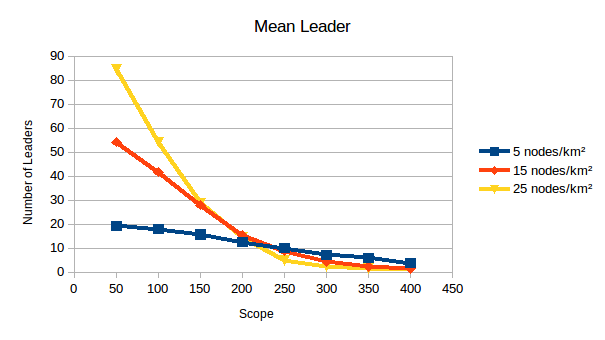
\includegraphics[width=\textwidth]{mean_leader.png}
\caption{Mean Leader}
\label{ML}
\end{figure}

Toutes les courbes sont décroissantes mais plus la densité est élevée, plus la courbe décroit vite. Cela semble cohérent puisqu'à faible densité, même si on augmente la portée, on aura de plus en plus de composantes connexes, mais quand même relativement peu. Plus on augmente la densité, plus on augmente la chance de former des composantes connexes qui contiendront presque tous les noeuds. 


\subsection{Question 5}

Cela signifie qu'à partir d'un certain seuil, la portée est assez grande pour qu'une grande partie des noeuds forment une composante connexe. Il ne sert donc à rien d'émettre à une portée plus importante.

\end{document}
